\begin{frame}{痛点}{手工精排 beamer 又慢又累}
  \begin{columns}[c,onlytextwidth]
    \column{0.54\textwidth}
      手工精排一套组会 beamer，往往\textbf{一晚上就没了}：逐页对齐图文、反复编译看溢出、字号留白来回试。

      \medskip
      \begin{itemize}
        \item 想清楚“讲什么”只占两成精力，\textbf{八成耗在排版}
        \item 改一张图，整页又得重排
      \end{itemize}

      \bigskip
      \alert{这套 \texttt{make-slides} skill 把分工反过来：你定主线，AI 干精排。}
    \column{0.46\textwidth}
      \begin{figure}\centering
        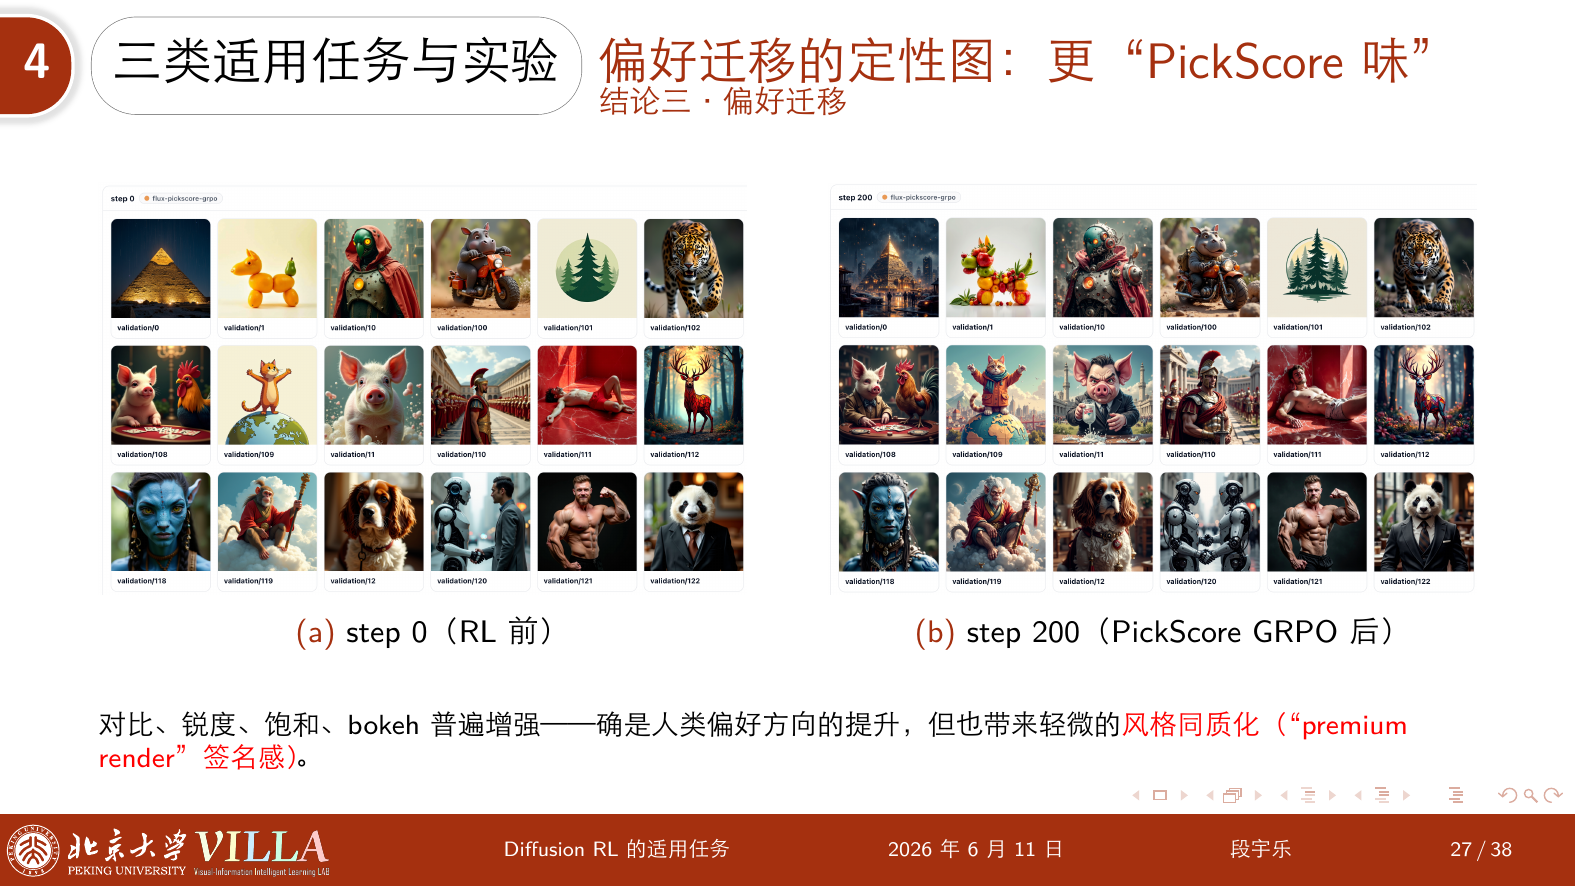
\includegraphics[width=\textwidth]{imgs/intro-show-qual.png}
        \caption{skill 的产出}
      \end{figure}
  \end{columns}
\end{frame}
